\documentclass{uc3mpracticas}

\usepackage{float}
\usepackage[export]{adjustbox}
\usepackage{caption}
\usepackage{subcaption}

%%%%%%%%%%%%%%%%%%%%%%%%%%%%%%%%%%%%%%%%%%%%%%%%%%%%%%%%%%%%%%%%%%%%%%%%%%%%%%%%
%%%                   Plantilla Prácticas UC3M                               %%%
%%%                Universidad Carlos III de Madrid                          %%%
%%%                   Alejandro Valverde Mahou                               %%%
%%%%%%%%%%%%%%%%%%%%%%%%%%%%%%%%%%%%%%%%%%%%%%%%%%%%%%%%%%%%%%%%%%%%%%%%%%%%%%%%

%Permitir cabeceras y pie de páginas personalizados
\pagestyle{fancy}

%Declarar formato de encabezado y pie de página de las páginas del documento
\fancypagestyle{doc}{
  %Cabecera
  \headerpr[1]{Trabajo Final}{}{Aprendizaje Automático}
  %Pie de Página
  \footerpr{}{}{{\thepage} de \pageref{LastPage}}
}

%Declarar formato de encabezado y pie del título e indice
\fancypagestyle{titu}{%
  %Cabecera
  \headerpr{}{}{}
  %Pie de Página
  \footerpr{}{}{}
}


\appto\frontmatter{\pagestyle{titu}}
\appto\mainmatter{\pagestyle{doc}}


\begin{document}
  %Comienzo formato título
  \frontmatter


  %Portada 1 (Centrado todo)
  \centeredtitle{Images/SmallLogo.jpg}{Grado en Ingeniería Informática}{Curso 2019-2020}{Aprendizaje Automático}{Trabajo Final}

  \vspace{40mm}

  \authors{Alba Reinders Sánchez}{100383444}{Alejandro Valverde Mahou}{100383383}{}{}{}{}

  \newpage


  %Índice
  \tableofcontents

  \listoffigures
  \newpage

  %Comienzo formato documento general
  \mainmatter


  \section{Definición del Problema}

  El problema a resolver es la clasificación de imágenes de muestras víricas para detectar el virus \textit{SARS-CoV-2}, también conocido como \textit{COVID-19}.

  \vspace{2mm}

  Esta idea nace de una propuesta realizada para el \textit{Hackathon} de la Comunidad de Madrid '\textit{Vence al virus}', el pasado 1 y 2 de Abril. La idea es identificar los pacientes infectados a través de las muestras víricas observadas con un microoscopio TEM (\textit{Transmission Electron Microscopes}), para así conseguir una prueba rápida, efectiva y de bajo coste.

  \vspace{2mm}

  Esta prueba deberá ser capaz de reconocer si el paciente está infectado por algún virus de la familia \textit{Coronaviridae} y, dado que existen muy pocos virus de esta familia que afectan a humanos, se podría asumir con cierta probabilidad que el paciente estaría infectado con el \textit{COVID-19}.

  \vspace{3mm}

  Se ha pensado resolver este problema a través de técnicas de aprendizaje automático porque se trata de un problema de clasificación. Dado que las imágenes usadas para el entrenamiento tendrán una clase asociada, se podrán usar técnicas de \textbf{aprendizaje supervisado}. De esta forma, se reduciría el tiempo necesario para clasificar cada una de las muestras, porque eliminaría la necesidad de los especialistas de tener que revisar cada una de las muestras para comprobar si el paciente está o no infectado.

  \vspace{2mm}

  Respecto a la viabilidad de la solución propuesta, se cree que supondría una reducción de coste y tiempo respecto a los medios actuales usados para detectar este virus. Sin embargo, la obtención de las imágenes necesarias para el entrenamiento puede ser complicada, ya que el microoscopio que se requiere para obtenerlas no se encuentra en todos los laboratorios de los hospitales.

  \vspace{2mm}

  La fiabilidad que se espera obtener de esta prueba es bastante elevada puesto que se conoce que los virus de la familia \textit{Coronaviridae} poseen una característica distintiva: suelen tener forma esférica y unas púas alredor de todo su cuerpo, de forma que facilitará la diferenciación de estos virus respecto a otros.

  \begin{figure}[H]
    \begin{center}
      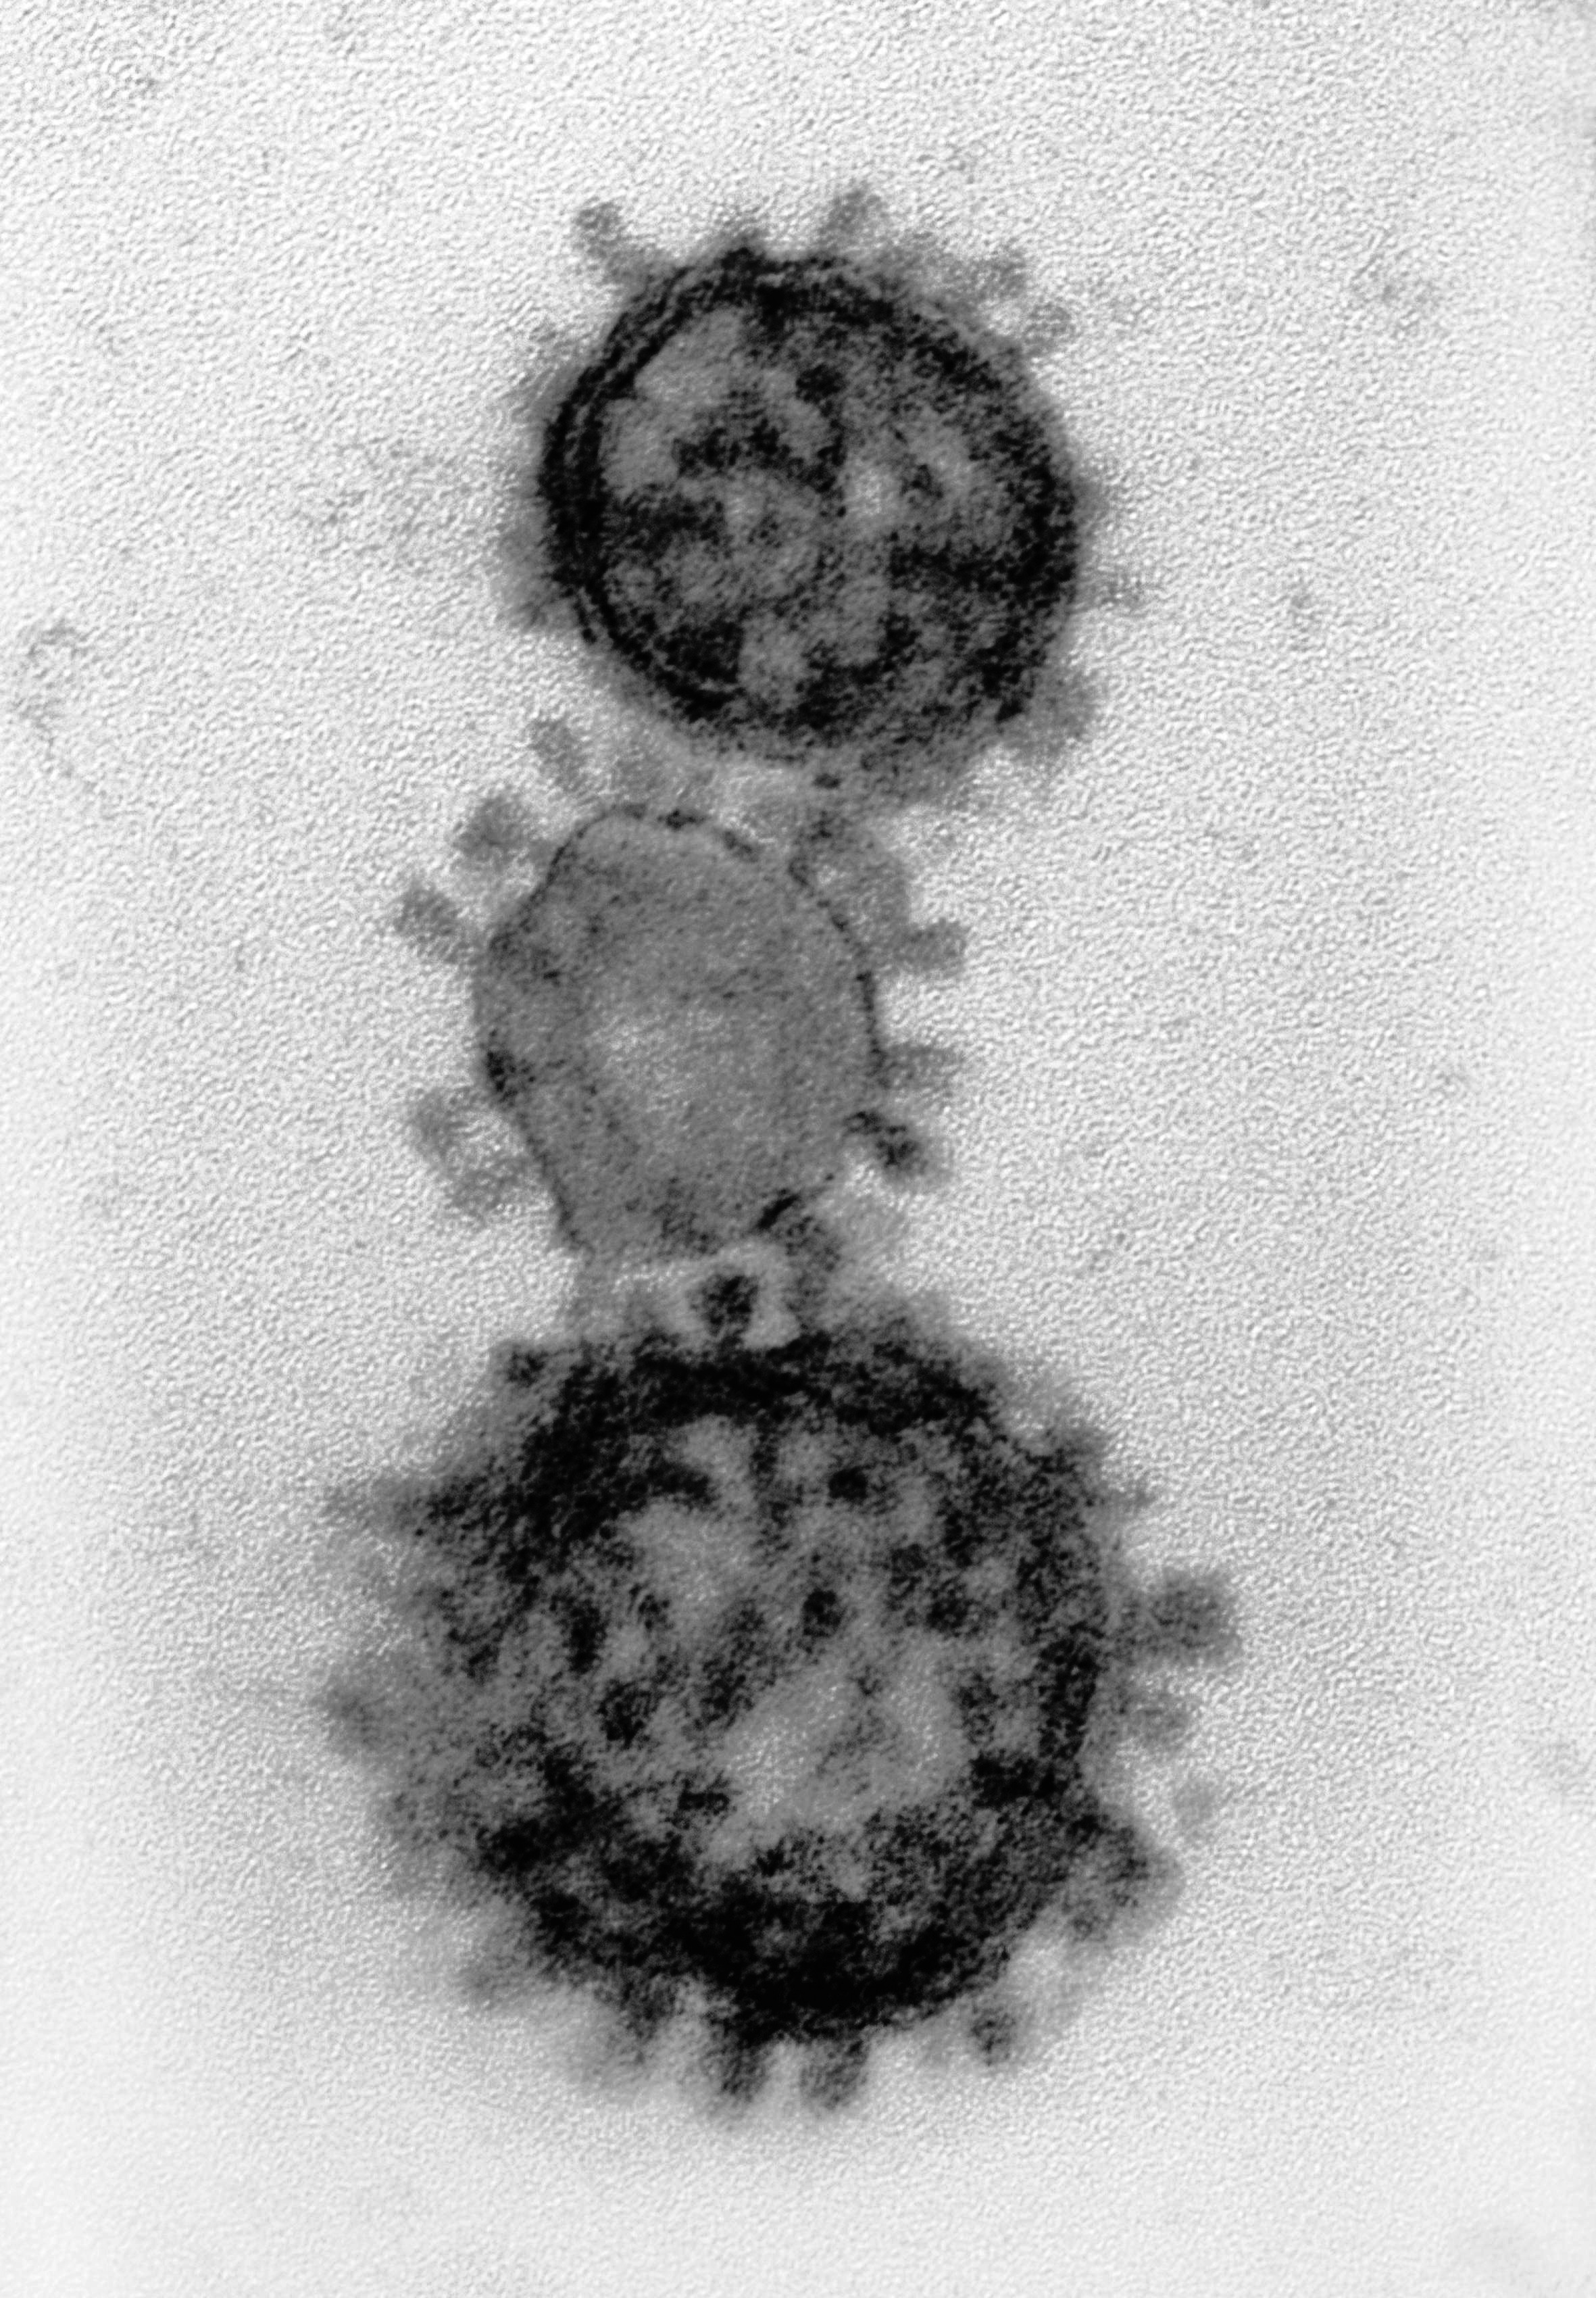
\includegraphics[angle=90,width=80mm, frame]{Images/coronaviridae/coronaviridae_0009.jpg}
      \caption{Muestra del virus \textit{COVID-19}}
    \end{center}
  \end{figure}

  El proceso que habría que llevar a cabo sería:

  \begin{enumerate}
    \item Recopilar un número de imágenes de muestras considerable entre las que se encuentren todo tipo de virus, entre ellos, el \textit{COVID-19}. Estas imágenes deberán estar previamente etiquetadas.
    \item Realizar un preprocesado a las imágenes.
    \item Entrenar el modelo de aprendizaje automático.
    \item Evaluar el modelo generado.
    \item Utilizar este modelo para clasificar nuevas imágenes.
  \end{enumerate}

  \vspace{2mm}

  Dado que el conjunto de datos son imágenes, se va a usar una \textbf{red de neuronas} para realizar la tarea de aprendizaje automático. Esta red tendrá que ser capaz de diferenciar muestras con \textit{COVID-19}, muestras con otros virus, y muestras vacías.

  \newpage

  \section{Datos y Obtención de Datos}

  El conjunto de datos que se usan para entrenar y evaluar el modelo son imágenes de muestras víricas clasificadas. Estas imágenes son tomadas por el microoscopio TEM, son en blanco y negro y de un tamaño variado. Estarán clasificadas en tres categorías: \textbf{COVID-19}, \textbf{otros virus} y \textbf{vacía}.

  \vspace{5mm}

  \begin{figure}[!h]
    \centering
    \begin{subfigure}[b]{0.3\textwidth}
      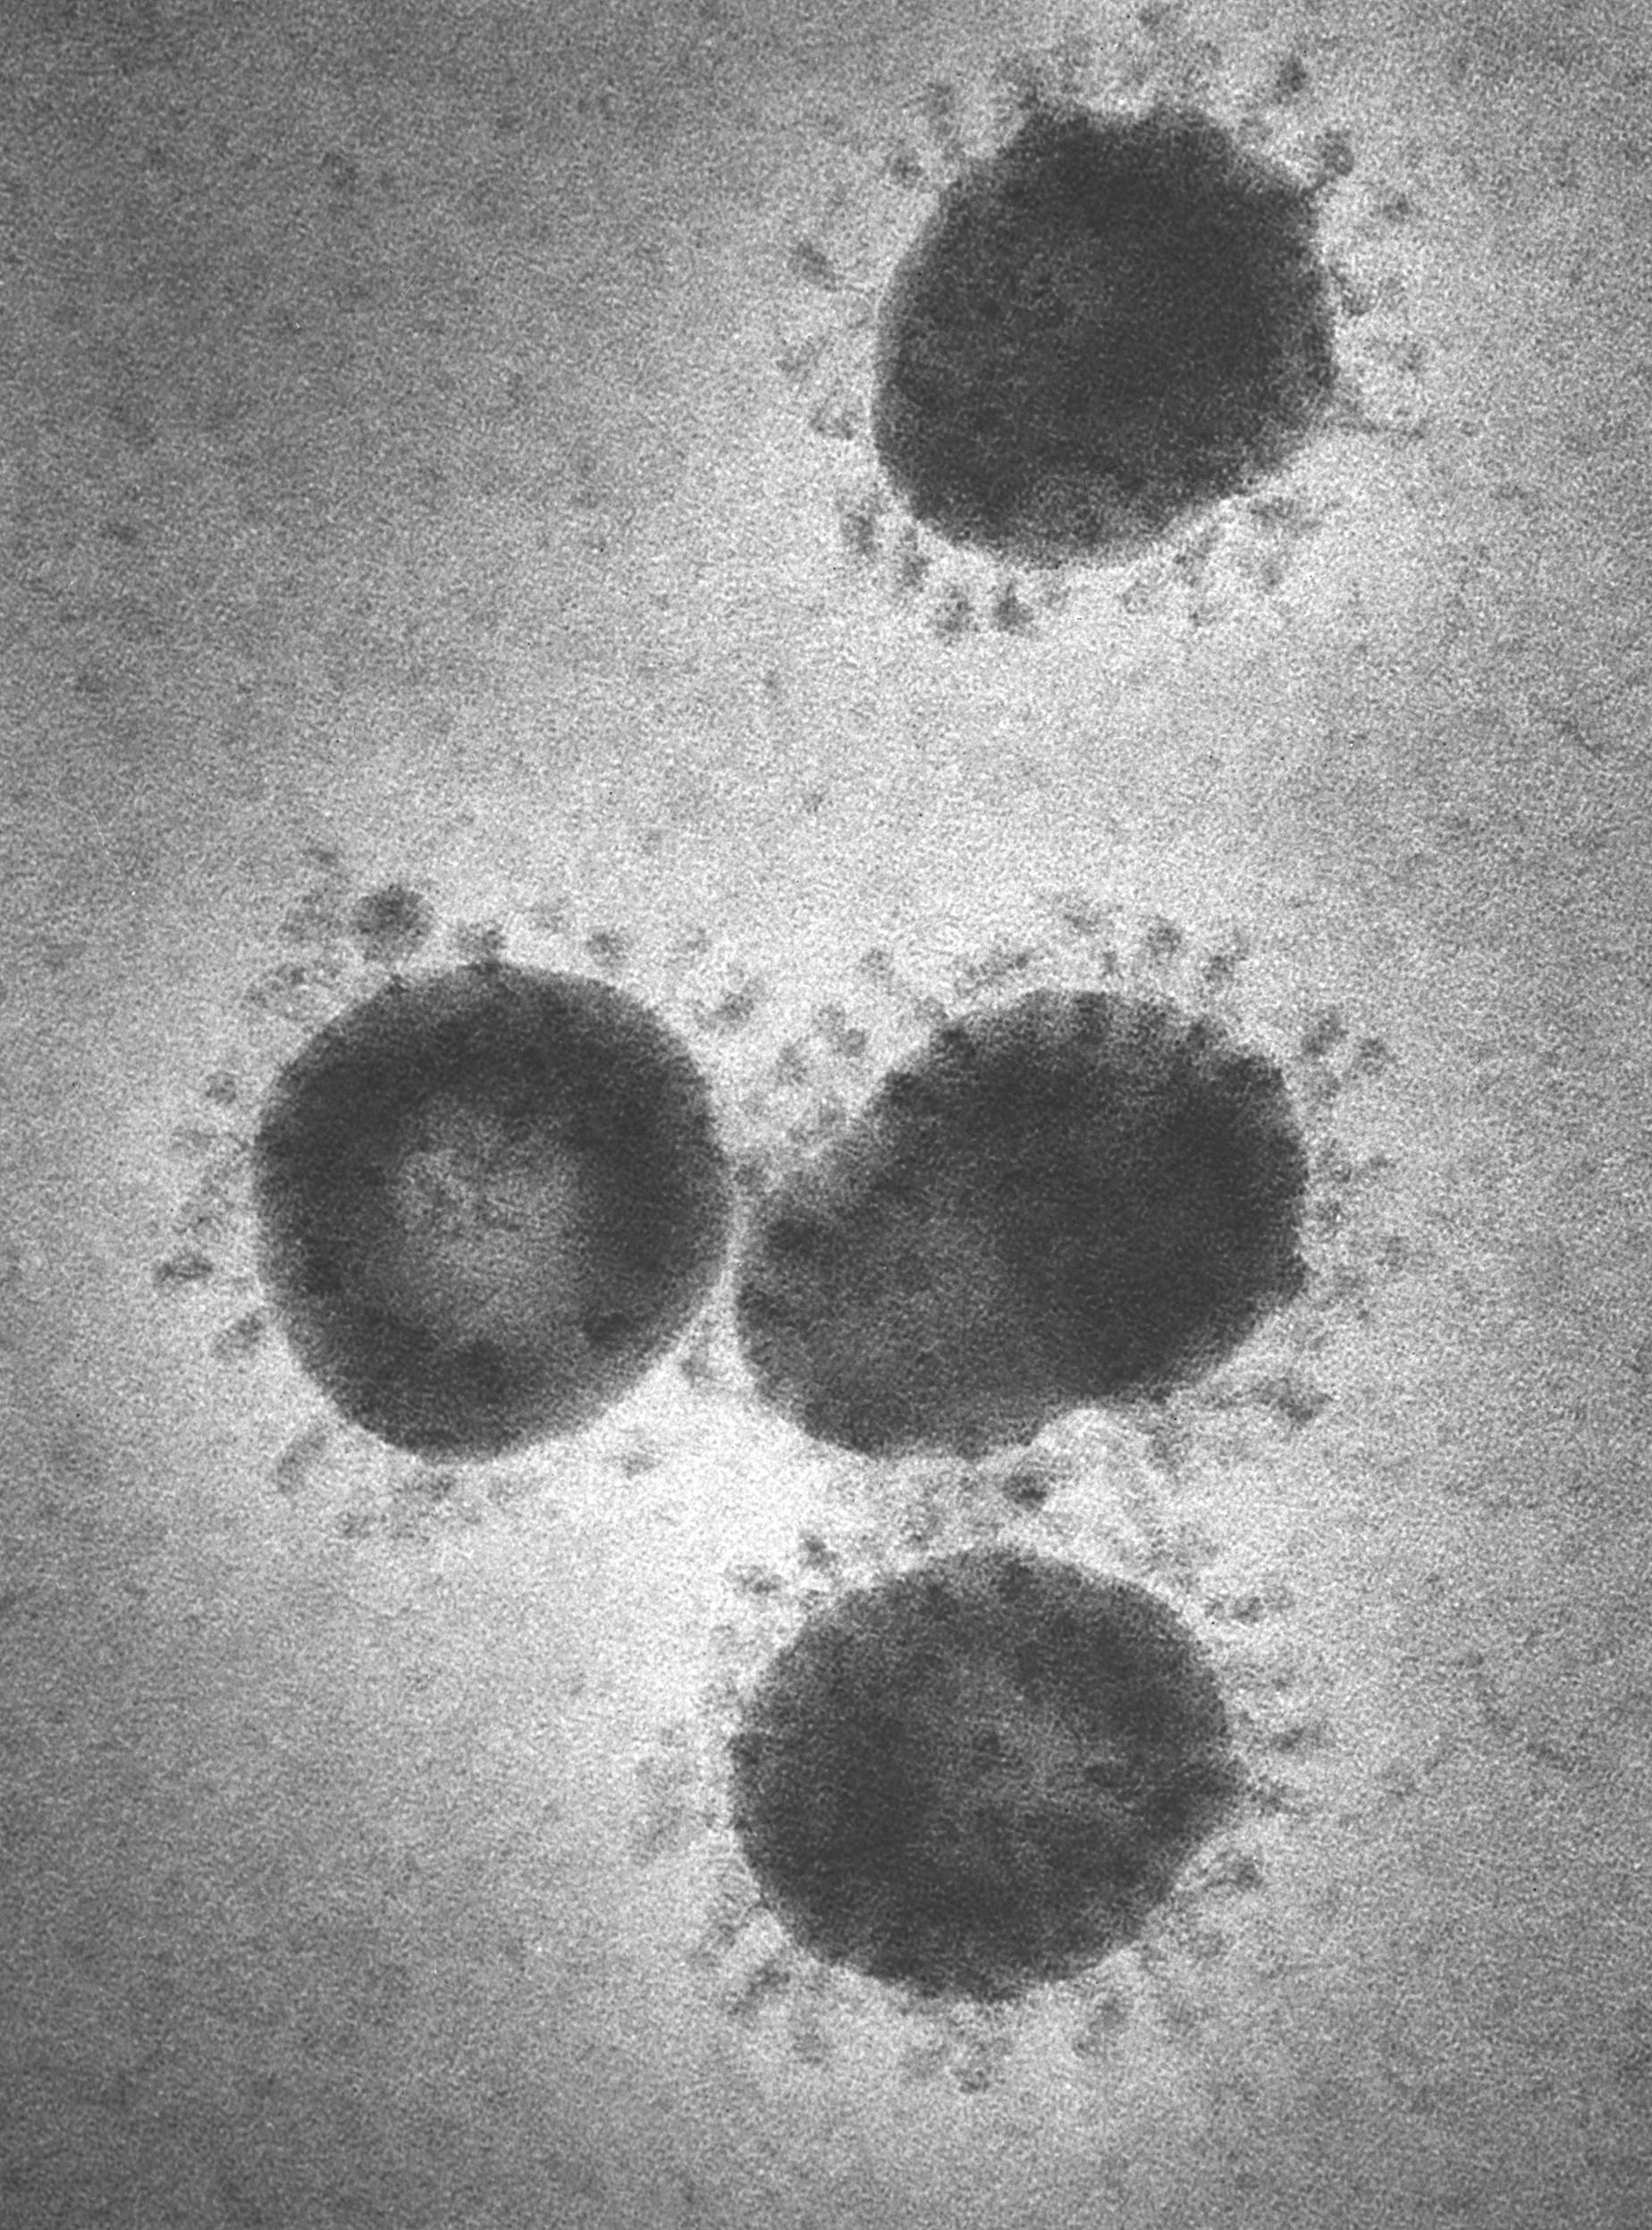
\includegraphics[angle=90, width=\textwidth, height=35mm, frame]{Images/coronaviridae/coronaviridae_0001.jpg}
      \caption{Muestra de \textit{COVID-19}}
    \end{subfigure}
    \hfill
    \begin{subfigure}[b]{0.3\textwidth}
      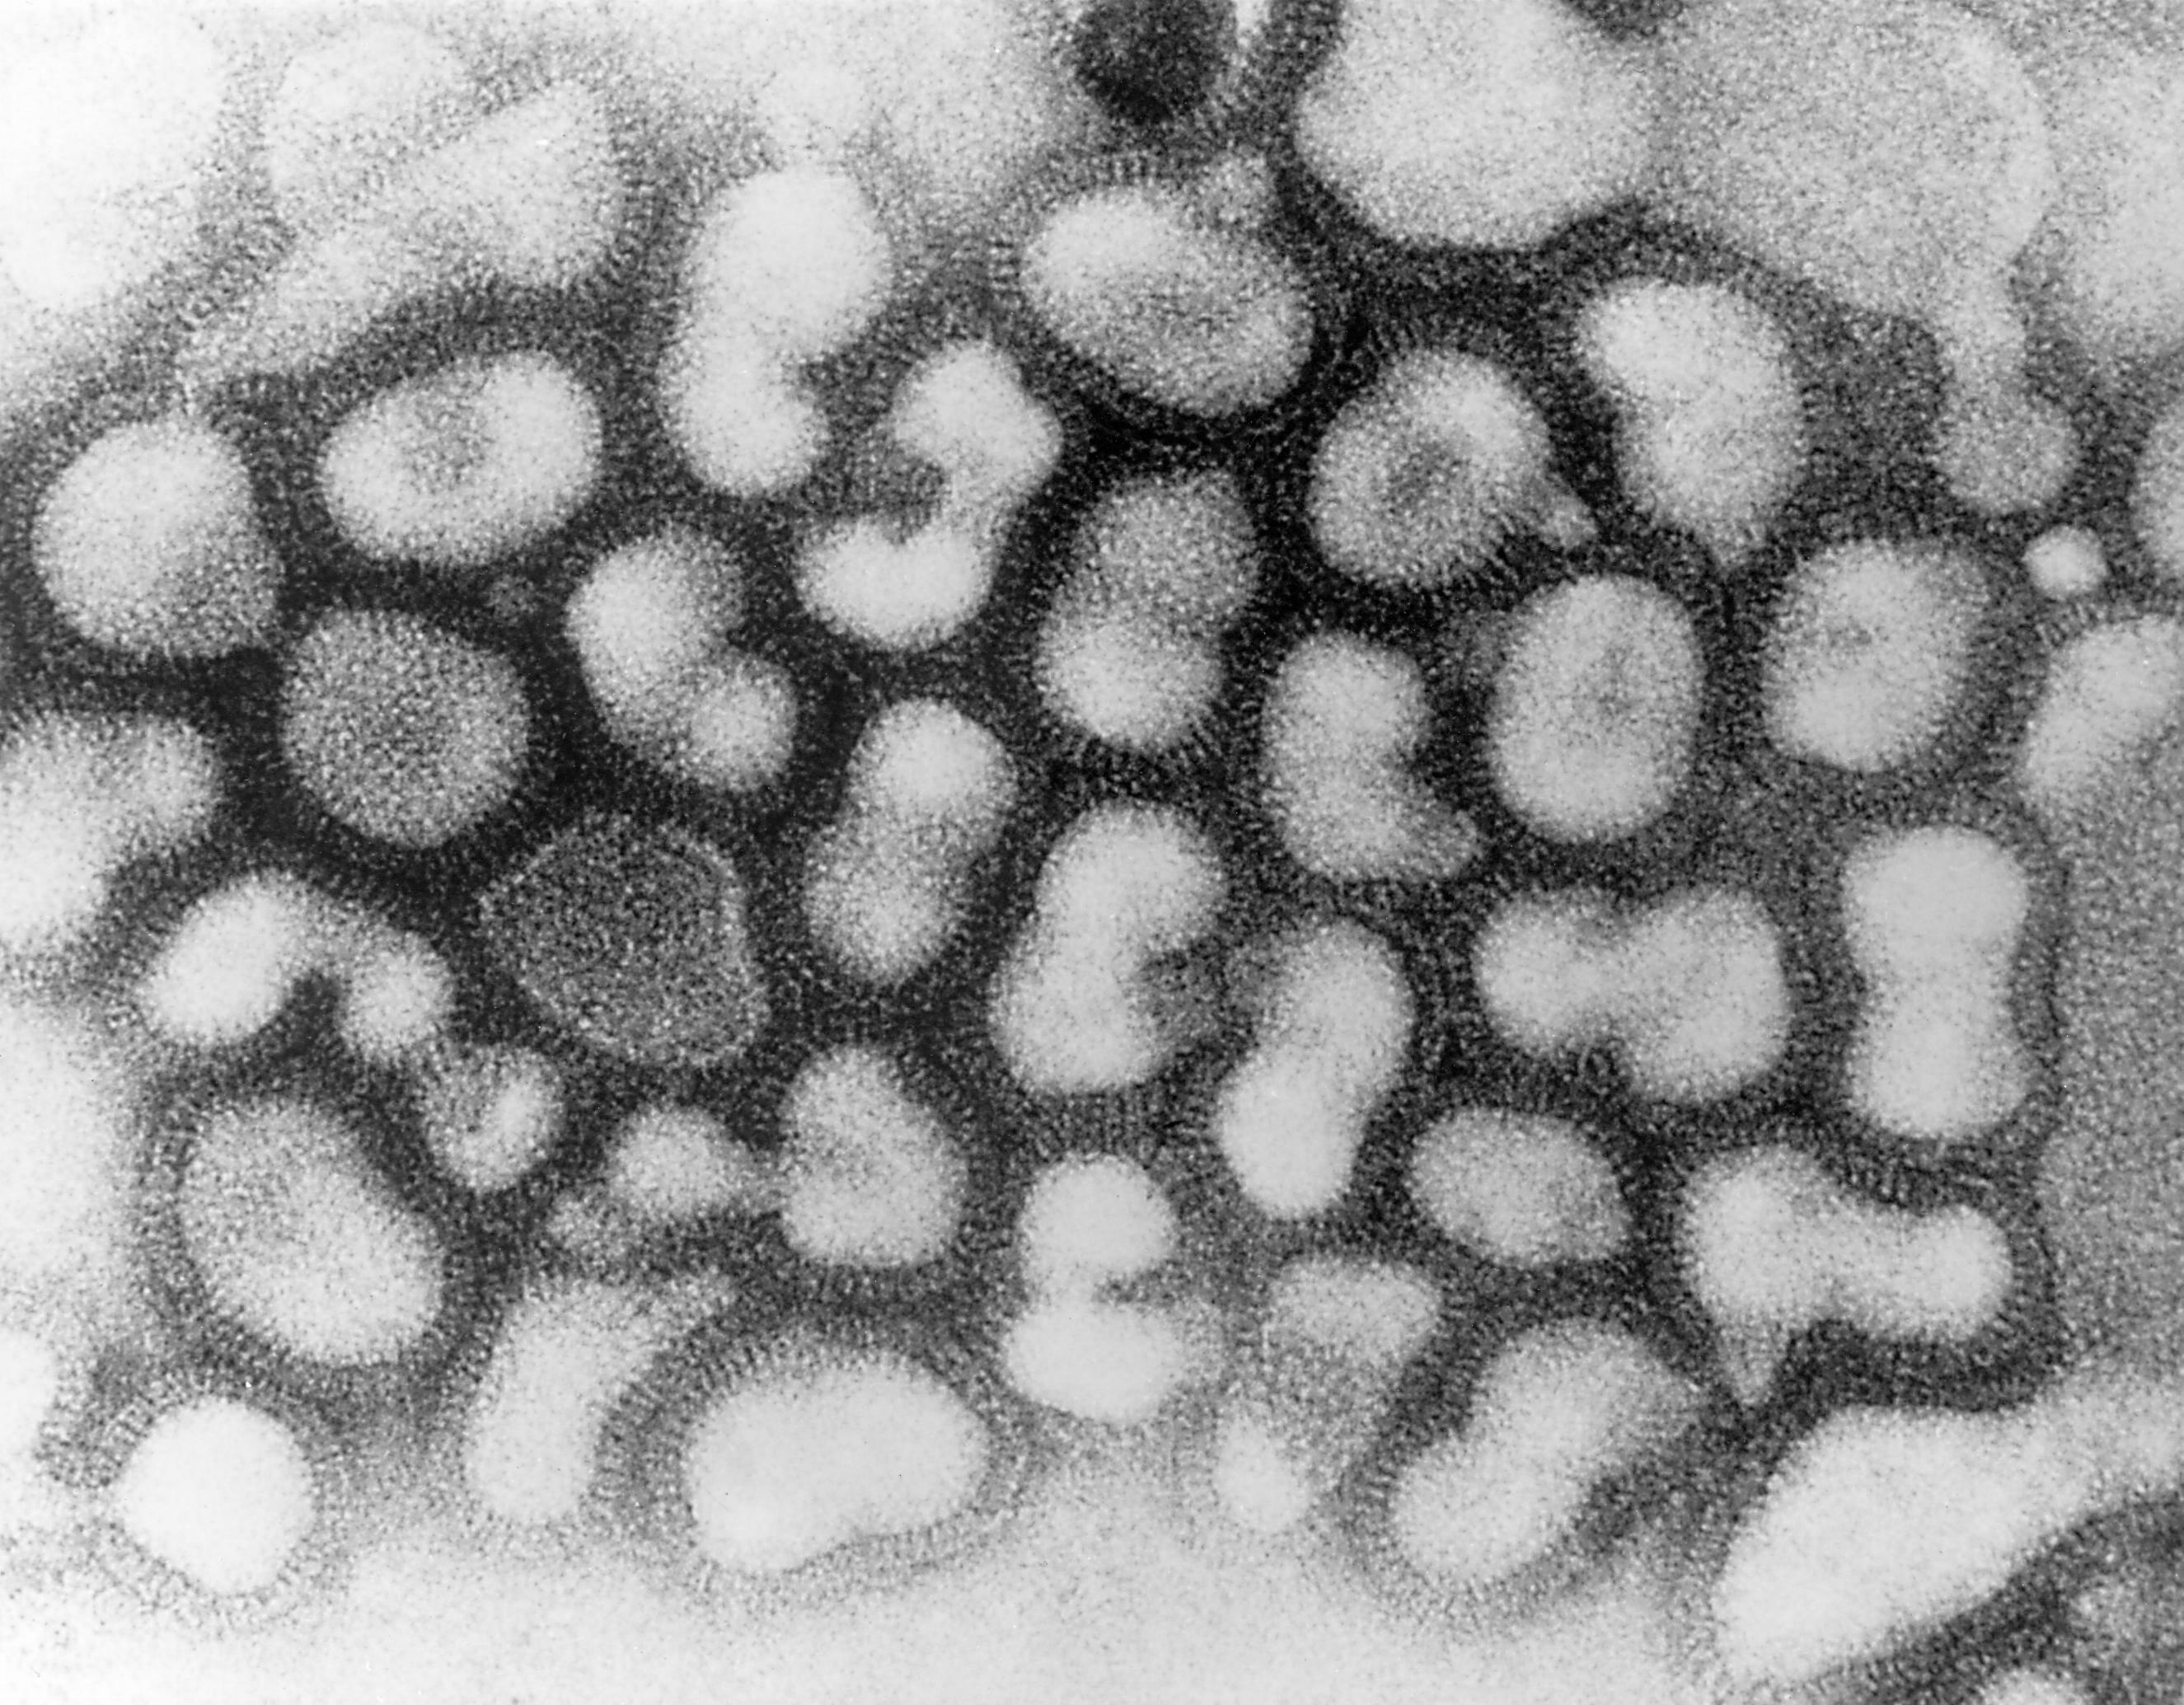
\includegraphics[width=\textwidth, height=35mm, frame]{Images/other/other_0021.jpg}
      \caption{Muestra de otros virus}
    \end{subfigure}
    \hfill
    \begin{subfigure}[b]{0.3\textwidth}
      
\includegraphics[width=\textwidth, height=35mm, frame]{Images/blank/blank_0019.jpg}
      \caption{Muestra vacía}
    \end{subfigure}

    \caption{Muestras víricas de ejemplo}
  \end{figure}


  \vspace{5mm}

  Los datos se obtienen del \textit{NIAID} (\textit{National Institute of Allergy and Infectious Diseases}) y de la \textit{Biblioteca Sanitaria Pública de EEUU}. También, y en base al \textit{Hackathon}, se estableció contacto con el \textit{CSIC} para conseguir mayor número de imágenes, aunque todavía no se han conseguido.

  \vspace{4mm}

  El problema principal de estas imágenes es su poca cantidad (alrededor de 50 imágenes de cada clase), por eso ha sido necesario contactar con el \textit{CSIC}. Ya que es de vital importancia conseguir un conjunto de imágenes lo suficientemente grande como para poder entrenar a la red de la mejor forma posible.

  \newpage

  \section{Preproceso de Datos}

  Dada la naturaleza de los datos, es necesario realizar ciertas transformaciones. La primera es que, a pesar de que las imágenes son de por sí en blanco y negro, había ciertos \textit{pixels} que se detectaban como formato \textit{RGB} y por tanto se han transformado a \textbf{escala de grises}.

  \vspace{2mm}

  A continuación, dado que las imágenes no tienen el mismo tamaño, se ha hecho un reescalado a todas las imágenes para que tengan un tamaño de \textbf{500x500px}.

  \vspace{4mm}

  Después, se dividió el conjunto de datos en \textbf{set de entrenamiento} y \textbf{set de evaluación}. Al hacer esta separación se ha decidido dividir en una proporción de 20\% evaluación (24 datos) y 80\% entrenamiento (102 datos).

  \vspace{4mm}

  Dado que el número de datos que se tienen es muy reducido, se va a optar por usar técnicas para aumentar el número de datos. Esto se hace para evitar el \textit{overfitting}, dado que con un número pequeño de datos, es más fácil que se produzca.

  \vspace{2mm}

  El aumento de datos se realizará en todas las imágenes del set de entrenamiento, para aumentar el máximo posible el número de datos. En un principio, no se va a realizar un aumento al set de evaluación.

  \vspace{2mm}

  Las técnicas de aumento de datos que se van a utilzar son: \textit{\textbf{rotación}}, \textit{\textbf{volteo}}, \textit{\textbf{traslación}} y \textit{\textbf{añadir ruido}}.

  \vspace{3mm}

  Otras técnicas que serían también útiles pero que no se van a implementar a menos que sean necesarias son: ampliar o alejar la imagen, rotaciones no solo de 90º y mezclar varias técnicas.

  \vspace{2mm}

  Estas técnicas se pueden aplicar a las imágenes debido a que no son especialmente simétricas, y por tanto, las nuevas imágenes generadas serán diferentes a las originales y permitirán a la red tener un mejor aprendizaje y reducir el \textit{overfitting}.

  \begin{figure}[!h]
    \centering
    \begin{subfigure}[b]{0.23\textwidth}
      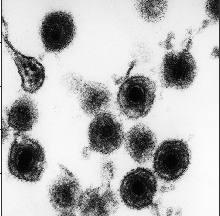
\includegraphics[width=\textwidth, frame]{Images/og.png}
      \caption{Imágen original}
    \end{subfigure}
    \hfill
    \begin{subfigure}[b]{0.23\textwidth}
      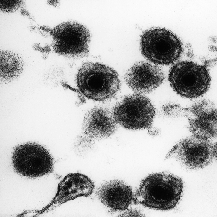
\includegraphics[width=\textwidth, frame]{Images/rot901.png}
      \caption{1 rotación de 90º}
    \end{subfigure}
    \hfill
    \begin{subfigure}[b]{0.23\textwidth}
      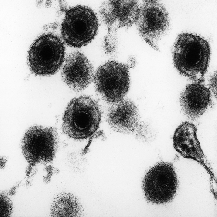
\includegraphics[width=\textwidth, frame]{Images/rot902.png}
      \caption{2 rotaciones de 90º}
    \end{subfigure}
    \hfill
    \begin{subfigure}[b]{0.23\textwidth}
      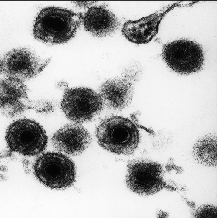
\includegraphics[width=\textwidth, frame]{Images/rot903.png}
      \caption{3 rotaciones de 90º}
    \end{subfigure}

    \caption{Imágenes generadas por \textbf{rotación}}
  \end{figure}


  \begin{figure}[!h]
    \centering
    \begin{subfigure}[b]{0.23\textwidth}
      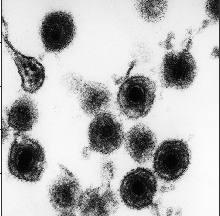
\includegraphics[width=\textwidth, frame]{Images/og.png}
      \caption{Imágen original}
    \end{subfigure}
    \hfill
    \begin{subfigure}[b]{0.23\textwidth}
      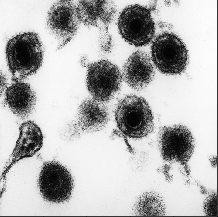
\includegraphics[width=\textwidth, frame]{Images/voltArrAbj.png}
      \caption{Volteo arriba-abajo}
    \end{subfigure}
    \hfill
    \begin{subfigure}[b]{0.23\textwidth}
      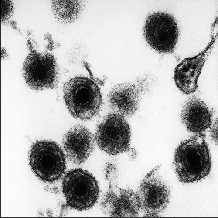
\includegraphics[width=\textwidth, frame]{Images/voltIzqDrch.png}
      \caption{Volteo izq-drch}
    \end{subfigure}
    \hfill
    \begin{subfigure}[b]{0.23\textwidth}
      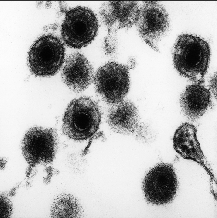
\includegraphics[width=\textwidth, frame]{Images/voltIDAA.png}
      \caption{Volteo combinado}
    \end{subfigure}

    \caption{Imágenes generadas por \textbf{volteo}}
  \end{figure}

  \begin{figure}[!h]
    \centering
    \begin{subfigure}[b]{0.18\textwidth}
      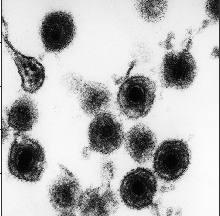
\includegraphics[width=\textwidth, frame]{Images/og.png}
      \caption{Imágen original}
    \end{subfigure}
    \hfill
    \begin{subfigure}[b]{0.18\textwidth}
      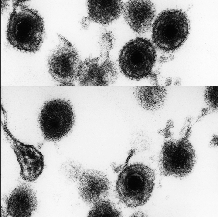
\includegraphics[width=\textwidth, frame]{Images/trasAbj.png}
      \caption{Traslación abajo}
    \end{subfigure}
    \hfill
    \begin{subfigure}[b]{0.18\textwidth}
      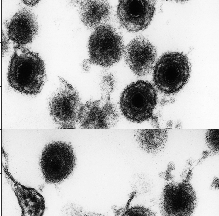
\includegraphics[width=\textwidth, frame]{Images/trasArr.png}
      \caption{Traslación arriba}
    \end{subfigure}
    \hfill
    \begin{subfigure}[b]{0.18\textwidth}
      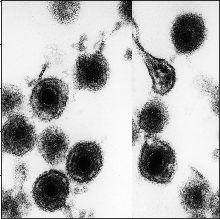
\includegraphics[width=\textwidth, frame]{Images/trasIzq.png}
      \caption{Traslación izq}
    \end{subfigure}
    \hfill
    \begin{subfigure}[b]{0.18\textwidth}
      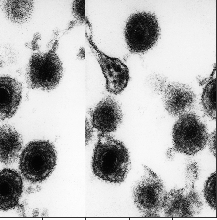
\includegraphics[width=\textwidth, frame]{Images/trasDrch.png}
      \caption{Traslación derecha}
    \end{subfigure}

    \caption{Imágenes generadas por \textbf{traslación}}
  \end{figure}

  \begin{figure}[!h]

    \hspace{0.16\textwidth}
    \begin{subfigure}[H]{0.25\textwidth}
      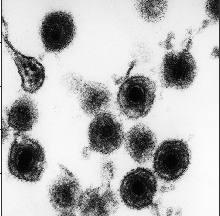
\includegraphics[width=\textwidth, frame]{Images/og.png}
      \caption{Imágen original}
    \end{subfigure}
    \hspace{0.16\textwidth}
    \begin{subfigure}[H]{0.25\textwidth}
      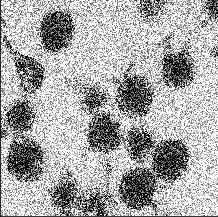
\includegraphics[width=\textwidth, frame]{Images/noise.png}
      \caption{Imágen con ruido}
    \end{subfigure}

    \caption{Imágenes generadas con \textbf{ruido}}
  \end{figure}


    \newpage

  \section{Modelado}

  Como la tarea definida es una clasificación de imágenes, el algoritmo que se va a usar es una \textbf{red neuronal convolucional}. Esta es una red neuronal formada por la siguiente combinación de capas: convolucional, \textit{pooling} y densa. Estas redes son especialmente buenas en problemas relacionados con imágenes, porque son capaces de obtener características de las mismas, útil en esta clasificación.

  \vspace{3mm}

  La arquitectura básica consiste en varias capas convolucionales y de \textit{pooling} intercaladas, seguidas de una o varias capas densas.

  \begin{itemize}
    \item \textbf{Convolucional}: capa formada por neuronas convolucionales que se encargan de procesar matrices de entrada con una operación sobre ellas, en lugar de un único valor numérico. Usan un \textit{kernel} para recorrer las matrices e ir extrayendo de ellas distintas características, con el objetivo de conseguir información útil. En este caso, la matriz es los valores de los \textit{pixels} de las imágenes. La salida de cada neurona de una capa convolucional es:

    \begin{center}
      $ \displaystyle Y_{j}=f\left(b_{j}+\sum_{i}K_{ij}\otimes Y_{i}\right) $
    \end{center}


    Donde $\displaystyle Y_{j}$ es la salida de una neurona $\displaystyle j$ y consiste en una matriz que se calcula a través de la combinación lineal de las salidas de las neuronas en la capa anterior ($\displaystyle Y_{i}$), cada una de ellas operadas con el \textit{kernel} $\displaystyle K_{ij}$ correspondiente a esa conexión. Esta cantidad se suma a una constante $\displaystyle b_{j}$ y luego se pasa por la función de activación de la neurona ($\displaystyle f()$).

    \vspace{2mm}

    La anterior operación se realiza de la siguiente manera:

    \begin{figure}[H]
      \centering
      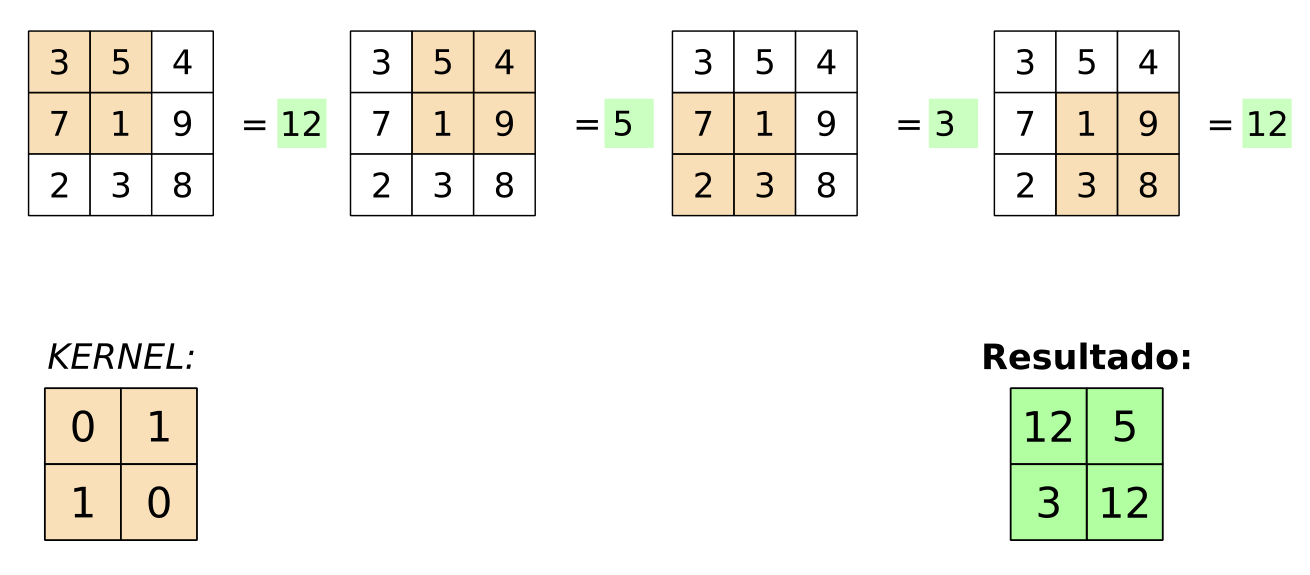
\includegraphics[width=\textwidth]{Images/kernel.png}
      \caption{Operación convolucional en una matriz 3x3 con un \textit{kernel} de 2x2}
    \end{figure}

    Donde el \textit{kernel} se inicializa aleatoriamente, y va variando sus valores a lo largo del entrenamiento, buscando la configuración ideal.

    \vspace{2mm}

    Con esto se consigue reducir el tamaño de la matriz de forma que se van consiguiendo las características más relevantes de cada sección en cada capa.


    \item \textbf{\textit{Pooling}}: capa encargada de reducir el tamaño de la matriz de entrada drásticamente, realizando una operación para resumir las características de una región. En concreto \textit{max-pooling}, encuentra el valor máximo dentro de un grupo de píxeles.

    \item \textbf{Densa}: capa formada por neuronas completamente enlazadas. La salida de cada neurona dentro de una capa densa depende de su entrada y sus pesos asociados, y sigue la siguiemte fórmula:

    \begin{center}
      $ \displaystyle Y_{j}=f\left(b_{j}+\sum_{i}\omega_{ij} \cdot Y_{i}\right)$
    \end{center}


    Donde $\displaystyle Y_{j}$ es la salida de una neurona $\displaystyle j$ y consiste en un valor que se calcula a través de la multiplicación de las salidas de las neuronas en la capa anterior ($\displaystyle Y_{i}$), cada una de ellas operadas con el peso asociado a la neurona $\omega_{ij}$. Este valor se suma a una constante $\displaystyle b_{j}$ y luego se pasa por la función de activación de la neurona ($\displaystyle f()$).

  \end{itemize}

  Además, y para conseguir el correcto funcionamiento de la red, es necesario añadir capas adicionales auxiliares:

  \begin{itemize}
    \item \textbf{\textit{Flatten}}: esta capa no aporta información a la red, y su única funcionalidad es la de hacer de puente entre las capas convolucionales y las capas densas, ya que tanto las entradas como las salidas de las capas convolucionales consisten en vectores tridimensionales, mientras que las capas densas trabajan con vectores unidimensionales. Por tanto, esta capa transforma este vector tridimensional '\textit{aplanándolo}', es decir, poniendo todos sus datos de forma consecutiva, para que la capa densa pueda utilizarlos.

    \item \textbf{\textit{Dropout}}: es una forma de regularizar el entrenamiento de la red. Sirve para prevenir el \textit{overfitting} de forma rápida y fácil.

    \item \textbf{\textit{Batch Normalization}}: normaliza los valor de la función de activación en una capa oculta. Así se evitan pesos fuera de rango, permite una tasa de aprendizaje más alta y reduce el \textit{overfitting}.

  \end{itemize}
  % Justificar el tipo de algoritmo adecuado para la/s tarea/s definida/s.
  %
  % Breve descripcion de la tecnica o tecnicas de aprendizaje automatico que se utilizarıan para resolverel problema.
  %
  % Describir como se plantearıa la seleccion de parametros
  % ¿Que parametros podrıan ser mas relevantes?
  % ¿Que factores se consideran para la seleccion de parametros?
  %
  % Describir si es necesaria alguna preparacion adicional de los datos especıfica para la/s tecnica/selegida/s.

  \newpage

  \begin{figure}[H]
    \centering
    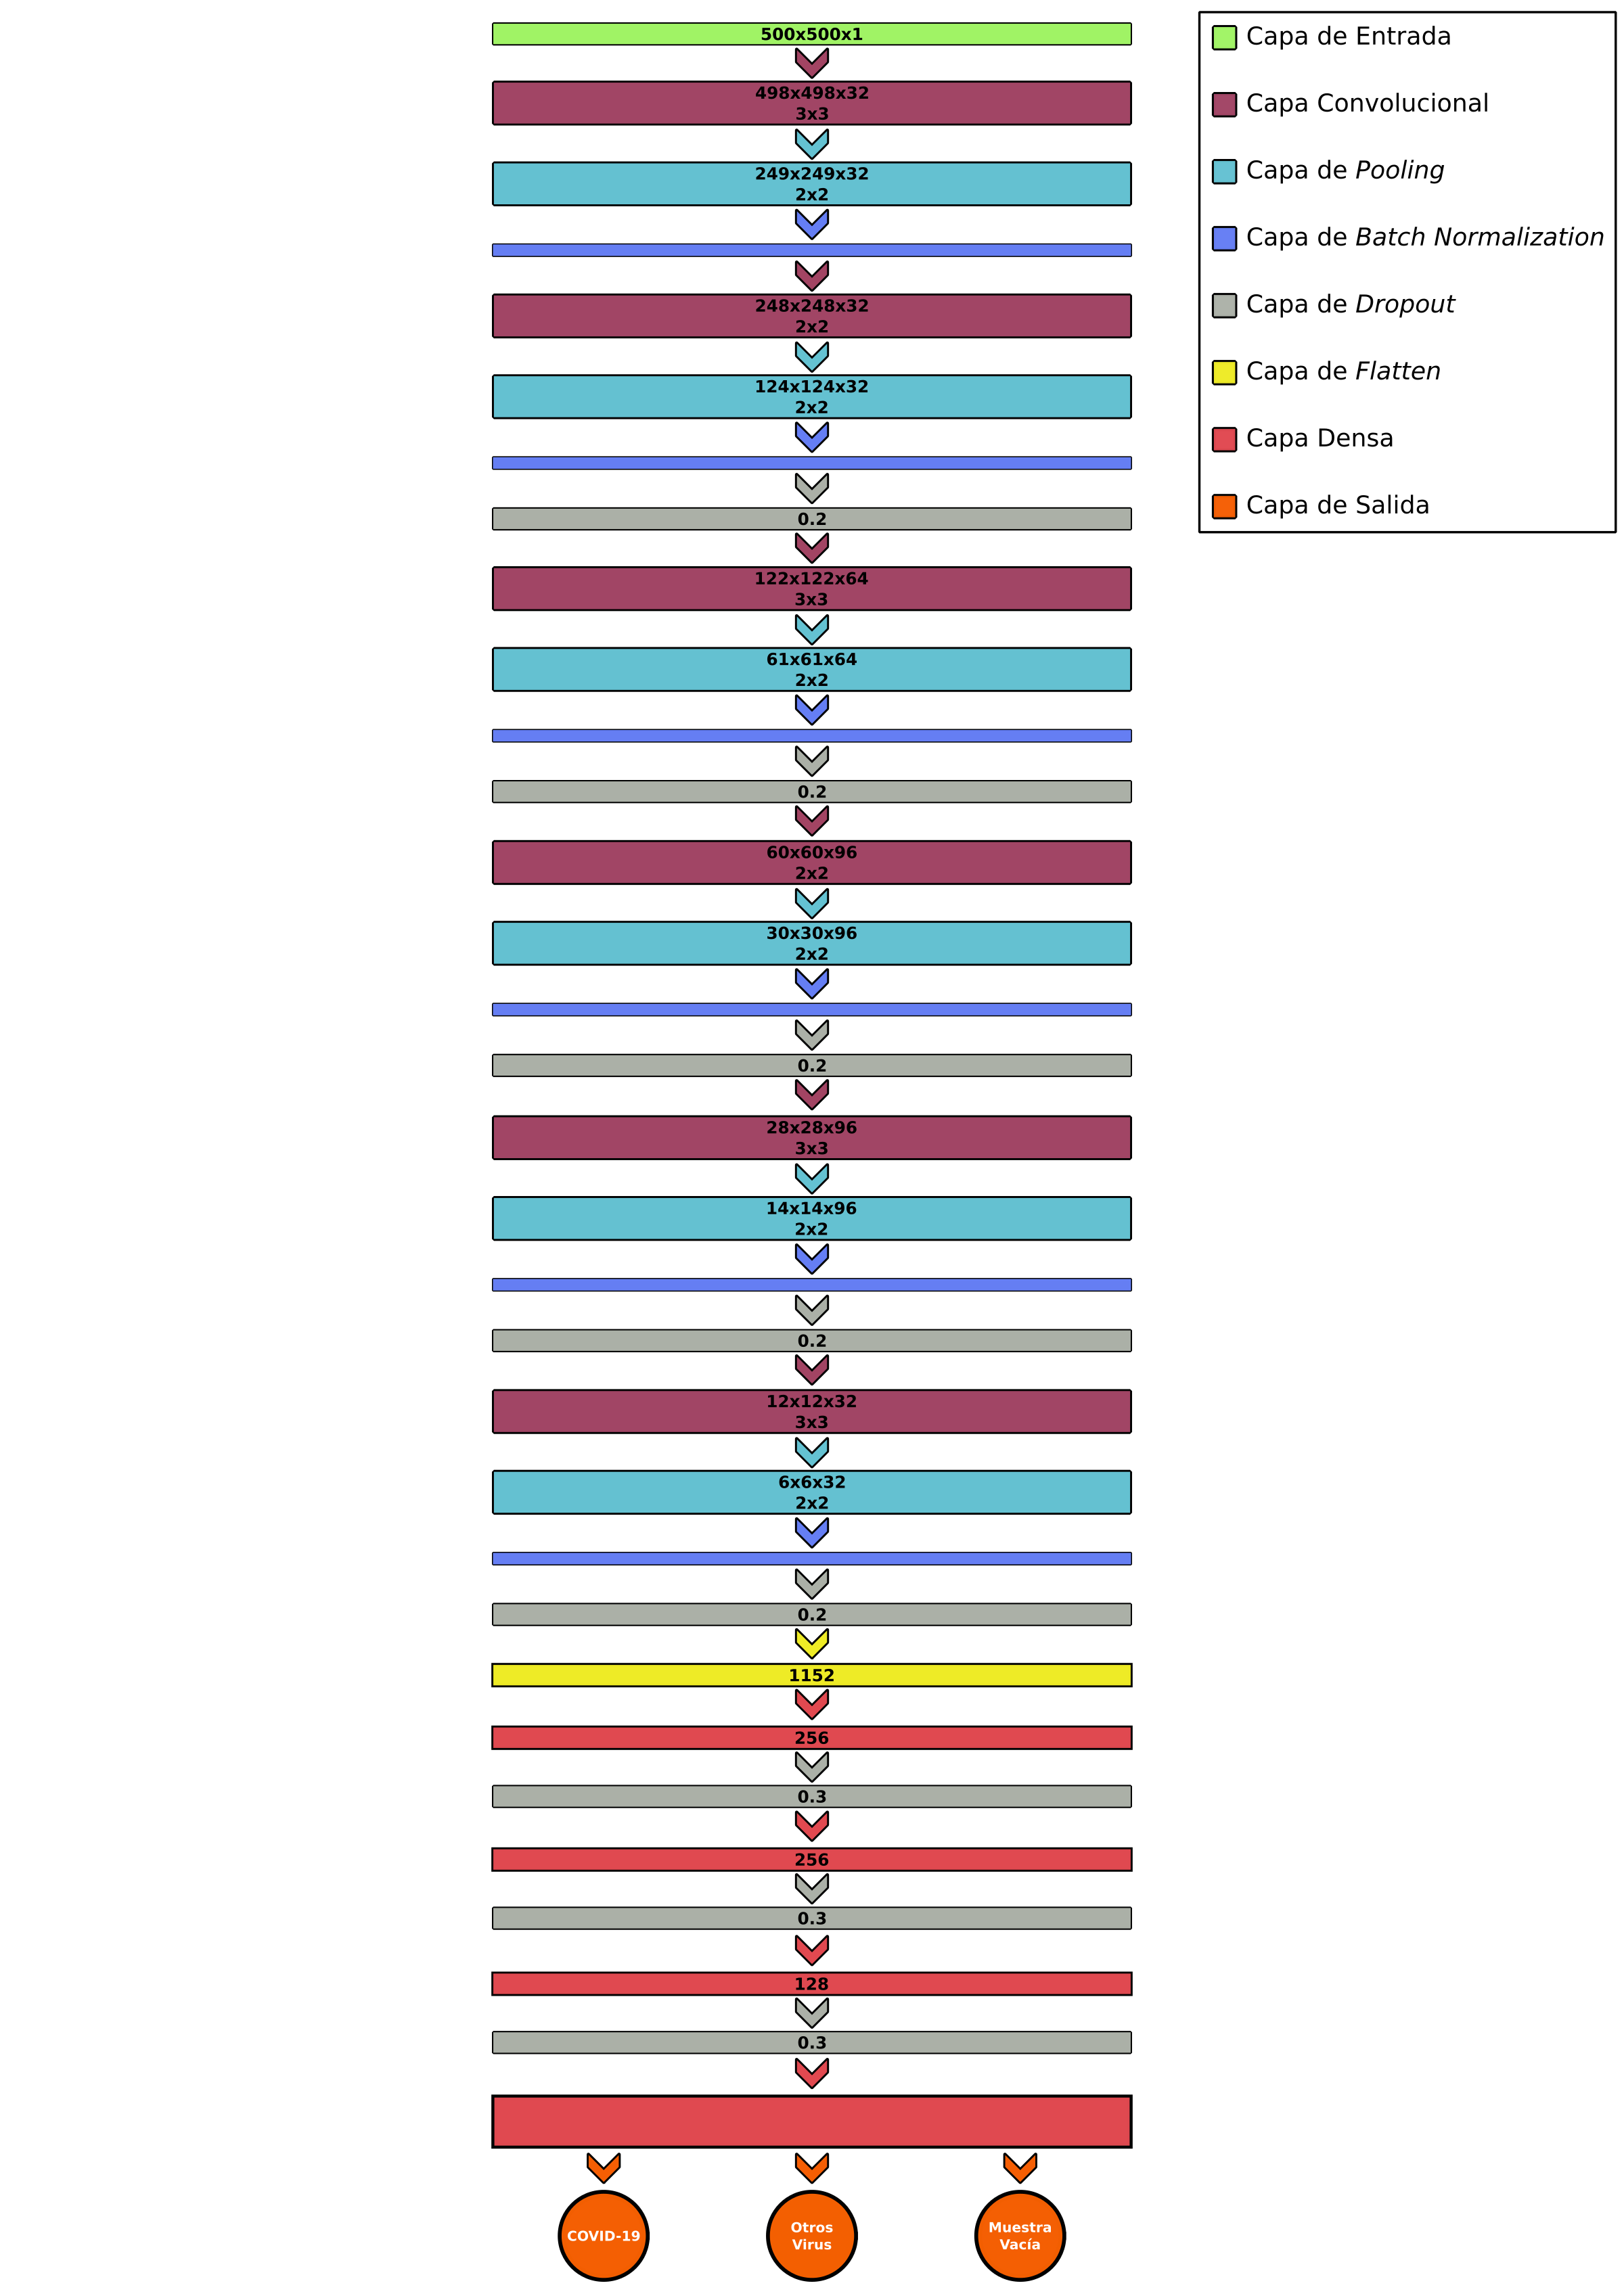
\includegraphics[width=\textwidth]{Images/CNN.png}
    \caption{Arquitectura de la red neuronal}
  \end{figure}

  \newpage

  \section{Evaluación}

  \newpage
  \section{Uso}








\end{document}
